\documentclass[12pt,fleqn]{article}
\setlength{\parindent}{0pt}
\usepackage{graphicx}
\usepackage{listings}
\usepackage[latin5]{inputenc}
\setlength{\parskip}{8pt}
\setlength{\parsep}{0pt}
\setlength{\headsep}{0pt}
\setlength{\topskip}{0pt}
\setlength{\topmargin}{0pt}
\setlength{\topsep}{0pt}
\setlength{\partopsep}{0pt}
\setlength{\mathindent}{0cm}

\begin{document}
MIT OCW Cok Degiskenli Calculus - Ders 6

Bir onceki derste cycloid konusunu isledik. 

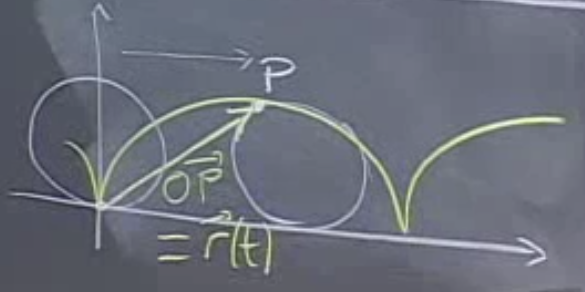
\includegraphics[height=4cm]{6_1.png}

Hareket eden bir noktanin pozisyonu

\[ (x(t), y(t), z(t)) \]

Bu noktayi takip etmenin diger yollarindan biri onu pozisyonu vektoru
olarak gormek, ki bu vektorun bilesenleri noktanin kordinatlari. 

\[ \vec{r}(t) = <x(t),y(t),z(t)> \]

Vektor orijin (baslangic) noktasindan gelinen noktayi isaret eden bir
vektor (resimde $\vec{OP}$). 

Onceki dersteki cycloid problemimiz icin, tekerlek yaricapi 1 olsun ve
birim hizda ilerliyor olalim, ki boylece aci $\theta$ ve zaman ayni sey
haline gelsin

\[ \vec{r}(t) = <t-sin(t), 1-cos(t) \]











\end{document}
